\documentclass[../report.tex]{subfiles}
\graphicspath{{\subfix{../image/}}}

\begin{document}
\maketitle

\subsection{PWM}
In order to control the drive and mast motors we used the L298n motor drivers which require 
a pwm signal for the speed selection. 
We control the speed of the motors by changing the duty cycle of the signal, as the drivers 
take than the average in percentage and make that the output voltage. Then a signal with duty 
cycle of 50\% drives the motors with half the input voltage of the drivers or visualized: 

\begin{center}
  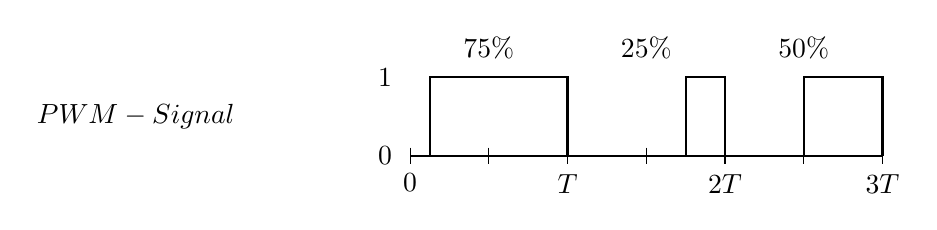
\begin{tikzpicture}
    \centering
    % Draw horizontal line
    \draw (0,0) -- (6,0);
    % Draw vertical lines
    \foreach \x in {0,1,2,3,4,5,6}
      \draw (\x cm,3pt) -- (\x cm,-3pt);
    % Draw PWM signal
    \draw[thick] (0,0) -- (0.25,0) -- (0.25,1) -- (2,1) -- (2,0)
                       -- (3.5,0) -- (3.5,1) -- (4,1) -- (4,0) 
                       -- (5,0) -- (5,1) -- (6,1) -- (6,0);

    \node[above=3pt] at (1,1) {$75\%$};
    \node[above=3pt] at (3,1) {$25\%$};
    \node[above=3pt] at (5,1) {$50\%$};


    \node[below=3pt] at (0,0) {$0$};
    \node[below=3pt] at (2,0) {$T$};
    \node[below=3pt] at (4,0) {$2T$};
    \node[below=3pt] at (6,0) {$3T$};
    \node[left=3pt] at (0,1) {$1$};
    \node[left=3pt] at (0,0) {$0$};

    \node[left=3pt] at (-2,0.5) {$PWM-Signal$};

\end{tikzpicture}  
\end{center}

\begin{center}
    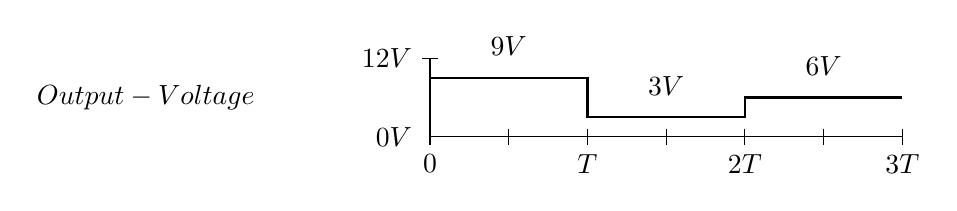
\begin{tikzpicture}
      \centering
      % Draw horizontal line
      \draw (0,0) -- (6,0);
      \draw (0,0) -- (0,1);
      \draw (-0.1,1)--(0.1,1);

      % Draw vertical lines
      \foreach \x in {0,1,2,3,4,5,6}
        \draw (\x cm,3pt) -- (\x cm,-3pt);
      % Draw PWM signal
      \draw[thick] (0,0.75) -- (2,0.75) -- (2,0.25) --
                   (4,0.25) -- (4,0.5)  -- (6,0.5);

      \node[above=3pt] at (1,0.8) {$9V$};
      \node[above=3pt] at (3,0.3) {$3V$};
      \node[above=3pt] at (5,0.55) {$6V$};
  
  
      \node[below=3pt] at (0,0) {$0$};
      \node[below=3pt] at (2,0) {$T$};
      \node[below=3pt] at (4,0) {$2T$};
      \node[below=3pt] at (6,0) {$3T$};

      \node[left=3pt] at (0,1) {$12V$};
      \node[left=3pt] at (0,0) {$0V$};
  
      \node[left=3pt] at (-2,0.5) {$Output-Voltage$};
  
  \end{tikzpicture}  
\end{center}
  
This can be implemented with the ESP32 by use of the Ledc library which allows 
for 8 independent PMW channels and on the fly adapting of duty cycle and frequency
resulting in seamless operations. 

\subsubsection{Configuring}
To configure a PWM signal we start by setting and enabling one of multiple timers,
most important here for us is the duty resolution as this later defines the accuracy 
and speed control of our signal. We choose a 8 bit resolution as we have worked with 
it in the first semester giving us now intuitive control and more accuracy was not needed. 
For testing purposes a 13bit resolution was tried and measured on the oscilloscope 
giving an impressive 50.004 \% duty cycle when set to 50\% through code.
\begin{lstlisting}[language=c, caption={Timer config}]
    // Prepare and then apply the LEDC PWM timer configuration
    ledc_timer_config_t ledc_timer = {
        .speed_mode       = LEDC_LOW_SPEED_MODE,
        .duty_resolution  = 8,// resolution in bit, 
        .timer_num        = 0, 
        .freq_hz          = 1000,
        .clk_cfg          = 0 // configures clock automatically 
    };
    ledc_timer_config(&ledc_timer);
\end{lstlisting}
Next we set the channel, dependent on the motor id and it can be noted, that multiple 
channels can run on one timer.
\begin{lstlisting}[language=c, caption={Channel config}]
    // Prepare and then apply the LEDC PWM channel configuration
    ledc_channel_config_t ledc_channel = {
        .speed_mode     = LEDC_LOW_SPEED_MODE, 
        .channel        = motor,
        .timer_sel      = LEDC_TIMER_0,
        .intr_type      = 0, // disable interrupts
        .gpio_num       = GPIO,
        .duty           = 128, //Set duty to 50% in 8 bit :  (2**8)*50% = 128
        .hpoint         = 0
    };
    ledc_channel_config(&ledc_channel);
\end{lstlisting}
As this would already start the PWM signal the duty cycle is set to 0 afterwards until needed with further 
instructions.
\subsubsection{Implementation}
After the initialization the firmware can use and change the PWM signals on the fly without interrupting
any other timer configurations by this: 
\begin{lstlisting}[language=c, caption={PWM Implementation}]
void pwm_set(int motor, int duty){
    ledc_set_duty(LEDC_LOW_SPEED_MODE, motor, duty);  
    ledc_update_duty(LEDC_LOW_SPEED_MODE, motor); 
    ledc_timer_resume(LEDC_LOW_SPEED_MODE, motor);
}
\end{lstlisting}
The pwm-set function is then used in other functions - the drive functions - these can be found in the \texttt{FL\_drive.h} header file in SPRO3-Firmware.
\end{document}